\documentclass[11pt]{article}\usepackage[]{graphicx}\usepackage[]{color}
% maxwidth is the original width if it is less than linewidth
% otherwise use linewidth (to make sure the graphics do not exceed the margin)
\makeatletter
\def\maxwidth{ %
  \ifdim\Gin@nat@width>\linewidth
    \linewidth
  \else
    \Gin@nat@width
  \fi
}
\makeatother

\definecolor{fgcolor}{rgb}{0.345, 0.345, 0.345}
\newcommand{\hlnum}[1]{\textcolor[rgb]{0.686,0.059,0.569}{#1}}%
\newcommand{\hlstr}[1]{\textcolor[rgb]{0.192,0.494,0.8}{#1}}%
\newcommand{\hlcom}[1]{\textcolor[rgb]{0.678,0.584,0.686}{\textit{#1}}}%
\newcommand{\hlopt}[1]{\textcolor[rgb]{0,0,0}{#1}}%
\newcommand{\hlstd}[1]{\textcolor[rgb]{0.345,0.345,0.345}{#1}}%
\newcommand{\hlkwa}[1]{\textcolor[rgb]{0.161,0.373,0.58}{\textbf{#1}}}%
\newcommand{\hlkwb}[1]{\textcolor[rgb]{0.69,0.353,0.396}{#1}}%
\newcommand{\hlkwc}[1]{\textcolor[rgb]{0.333,0.667,0.333}{#1}}%
\newcommand{\hlkwd}[1]{\textcolor[rgb]{0.737,0.353,0.396}{\textbf{#1}}}%
\let\hlipl\hlkwb

\usepackage{framed}
\makeatletter
\newenvironment{kframe}{%
 \def\at@end@of@kframe{}%
 \ifinner\ifhmode%
  \def\at@end@of@kframe{\end{minipage}}%
  \begin{minipage}{\columnwidth}%
 \fi\fi%
 \def\FrameCommand##1{\hskip\@totalleftmargin \hskip-\fboxsep
 \colorbox{shadecolor}{##1}\hskip-\fboxsep
     % There is no \\@totalrightmargin, so:
     \hskip-\linewidth \hskip-\@totalleftmargin \hskip\columnwidth}%
 \MakeFramed {\advance\hsize-\width
   \@totalleftmargin\z@ \linewidth\hsize
   \@setminipage}}%
 {\par\unskip\endMakeFramed%
 \at@end@of@kframe}
\makeatother

\definecolor{shadecolor}{rgb}{.97, .97, .97}
\definecolor{messagecolor}{rgb}{0, 0, 0}
\definecolor{warningcolor}{rgb}{1, 0, 1}
\definecolor{errorcolor}{rgb}{1, 0, 0}
\newenvironment{knitrout}{}{} % an empty environment to be redefined in TeX

\usepackage{alltt}
\usepackage{amsmath}
\usepackage{amssymb}
\usepackage{geometry}
\usepackage{graphicx}
\usepackage{fullpage}
\usepackage{enumerate}
\IfFileExists{upquote.sty}{\usepackage{upquote}}{}
\begin{document}
\setlength\parindent{0pt}

Lecture 5: Normal Distribution\\
Practice Problems\\
STAT 310, Spring 2021\\

\textbf{Exercise 1}.  Suppose $Z \sim N(\mu = 0, \sigma = 1)$ is a random variable following a standard normal distribution.  Use the R function \texttt{pnorm()} to compute the following probabilities:
\begin{enumerate}[(a)]
\item $P(Z < 1.4)$\\

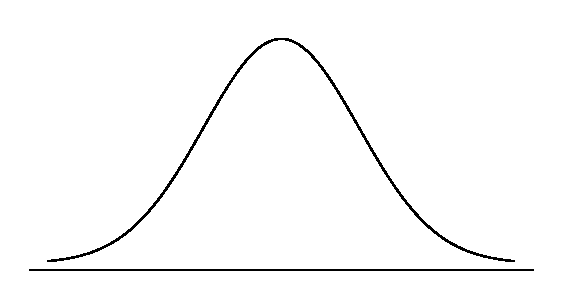
\includegraphics[scale=0.5]{figure/norm_draw.pdf}
\bigskip

\item $P(Z > 2.2)$

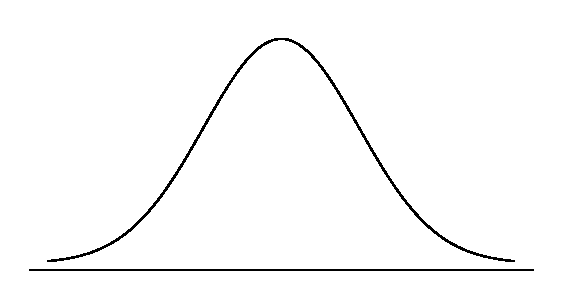
\includegraphics[scale=0.5]{figure/norm_draw.pdf}
\bigskip

\item $P(-0.5 < Z < 1.5)$

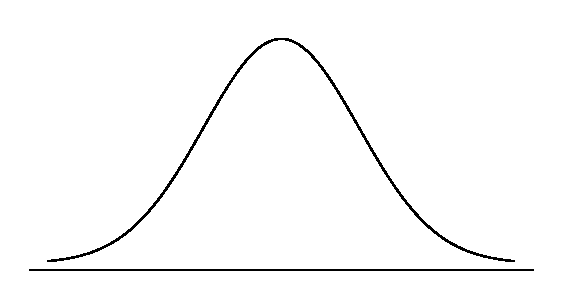
\includegraphics[scale=0.5]{figure/norm_draw.pdf}
\bigskip
\end{enumerate}

\textbf{Exercise 2}.  Use the R function \texttt{qnorm()} to find $85^{th}$ percentile of the standard normal distribution $N(\mu = 0, \sigma = 1)$.\\

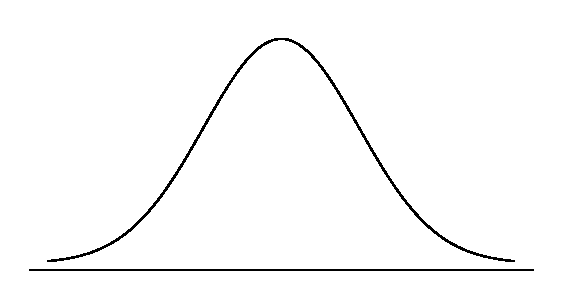
\includegraphics[scale=0.5]{figure/norm_draw.pdf}
\bigskip

\newpage

\textbf{Exercise 3}.  The SAT score $X$ closely follows a normal distribution with mean $\mu=1100$ and standard deviation $\sigma = 200$.  That is, $X \sim N(\mu = 1100, \sigma = 200)$
\begin{enumerate}[(a)]
\item About what percent of test takers score below a 750?\\
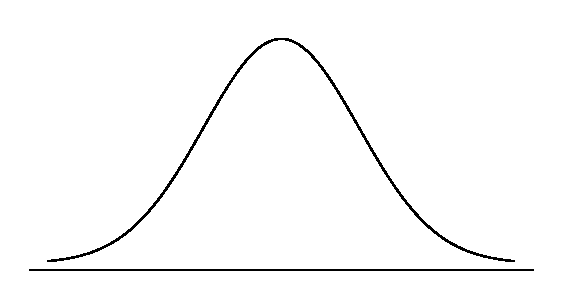
\includegraphics[scale=0.6]{figure/norm_draw.pdf}
\vspace{1cm}

\item About what percent of test takers score above a 1500?\\
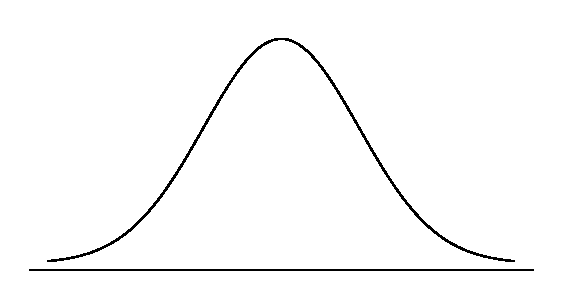
\includegraphics[scale=0.6]{figure/norm_draw.pdf}
\vspace{1cm}

\item About what percent of test takes score between 800 and 1400?\\
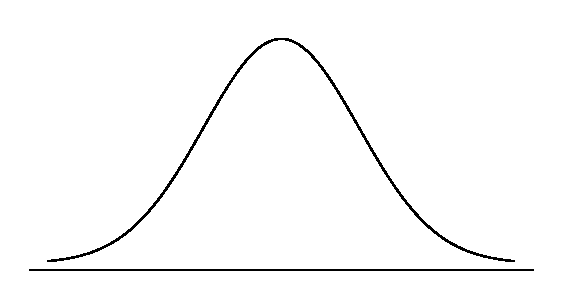
\includegraphics[scale=0.6]{figure/norm_draw.pdf}
\vspace{2cm}

\item What is the 95$^{th}$ percentile for SAT scores?\\
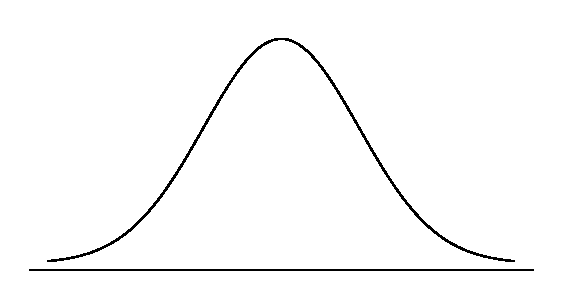
\includegraphics[scale=0.6]{figure/norm_draw.pdf}

\end{enumerate}

\end{document}
